\setAuthor{Oleg Košik}
\setRound{lahtine}
\setYear{2010}
\setNumber{G 8}
\setDifficulty{9}
\setTopic{Magnetism}

\prob{Laeng}
\begin{wrapfigure}[8]{r}{0.25\textwidth}
	\vspace{-2.5ex}
	
\includegraphics[width=\linewidth]{2010-lahg-08-laengu_joonis_ipe}
	\vspace{-6ex}
\end{wrapfigure}
Ruudukujulise ristlõikega ruumipiirkond on täidetud homogeense magnetväljaga
$B$ ning selle keskel asub osake massiga $m$ ja laenguga $q$, mis on alghetkel
paigal. Alates alghetkest iga ajavahemiku $T=\frac{\pi m}{qB}$ tagant lülitub
selles piirkonnas lühiajaliselt sisse elektriväli $E$ (kestusega $\tau \ll T$), mis
on suunatud risti magnetväljaga. Elektriväli võib muutuda kahes
režiimis: (i) olles iga kord suunatud joonisel näidatud suunas; (ii)
olles suunatud vaheldumisi kord joonisel näidatud suunas, kord vastupidises
suunas.\\
\osa Skitseerige osakese trajektoor mõlema režiimi korral.\\
\osa Kumma
režiimi korral väljub osake magnetväljaga piirkonnast kiiremini? Mitu korda
kiiremini?
Eeldage, et väljumisaeg on mõlemal juhul palju suurem kui $T$. Põhjendage vastust.

\hint
Magnetväljas liiguvad osakesed mööda ringjoont kiirusest sõltumatu perioodiga $t = \frac{2\pi m}{qB}$. Näeme, et ülesandes antud ajavahemik $T$ vastab poolele täistiirule. Antud tähelepanek võimaldab olukorra mugavamat skitseerimist. Iga kord kui elektriväli sisse lülitatakse, antakse osakesele väike elektriväljasihiline impulss.

\solu
Paneme tähele, et ajavahemik $T$ on võrdne poolega tsüklotronperioodist (ajaga, mis kulub sellel laengul magnetväljas täistiiru tegemiseks).
Seega antakse impulsimuut $\Delta p=Eq\tau$ iga kord kiirusega paralleelselt (ii) 
või antiparalleelselt (i). Seega hakkab juhtumil (ii) impulss kasvama lineaarses sõltuvuses lülituste arvuga $n=[t/T]$ (kus $t$ on vaadeldav
ajahetk ja nurksulud tähistavad täisosa): $p=Eq\tau[t/T]$. Et trajektoori kõverusraadius on võrdeline impulsiga, $R=v/\omega=p/qB$, siis 
kasvab kõverusraadius samuti lineaarselt $n$-ga, vt punktiirjoont joonisel. 
Juhtumil (i) paneb esimene jõuimpulss laengu liikuma, teine aga peatab liikumise. Tulemuseks on joonisel toodud laineline trajektoor (katkendjoon joonisel).
Tuginedes nendele trajektooridele saame teha tabeli osakese eemaldumuse $l = \max (x,y)$ jaoks $x$ või $y$-teljest erinevatel ajahetkedel.

\begin{tabular}{lllllllllll}
	$t/T$ & 0,5 & 1 & 1,5 & 2 & 2,5 & 3 & 3,5 & 4 & 4,5 & 5 \\
	$l/R$ (i) & 1 & 2 & 2 & 2 & 3 & 4 & 4 & 4 & 5 & 6 \\
	$l/R$ (ii) & 1 & 2 & 2 & 2 & 3 & 4 & 4 & 4 & 5 & 6
\end{tabular}

Nagu näha, toimub eemaldumine mõlemal juhul vaadeldavate ajahetkede jaoks täpselt ühekiiruselt. Siiski, kui kuubi poolküljepikkus ei ole 
mitte $R$-i täisarvkordne, siis väljub (i) juhtumi korral osake pisi-natuke varem. Sellest võib aru saada uurides võrdlevalt 
kauguse $l$ kasvufaase juhtumeil (i) ja (ii) ja juuresolevat joonist: antud ruudukujulise piirkonna jaoks väljumisaeg $2T+\Delta t$, kus
täiendav ajavahemik juhtumil (ii) $\Delta t=\pi \alpha/T$ juhtumil (i) $\Delta t=\pi \beta/T$.
Kuivõrd $\alpha > \beta$, siis saamegi järeldada, et juhtumil (i) väljub osake varem. On võimalik näha, et võrratus 
$\alpha > \beta$ kehtib peaaegu alati --- välja arvatud siis, kui kuubi külje pikkus on $R$-i paarisarvukordne.
Ülesandes antud eelduse $t\gg T$ tõttu muutub see väike väljumisaja erinevus tühiseks: aegade suhe sellel piirjuhul on 1.
\begin{center}
	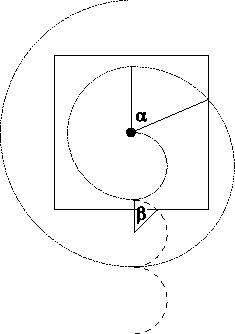
\includegraphics[width=0.35\textwidth]{2010-lahg-08-lah}
\end{center}
\probend